\documentclass{article}

\usepackage{graphicx}
\usepackage{graphpap}


\usepackage{fancyhdr}



%%%%%%%%%%%%%%%%%%%%%%%%%%%%%%%%%%%%%%%%5
%
%  Set Up Margins

%%%%%%%%%%%%%%%%%%%%%%%%%%%%%%%%%%%%%%%%%%%%%%%%%
% include file for:
%      Critical Page setup dimensions
%            DO NOT MODIFY
%       (for help see "Latex Line by Line" p 260)
%
\setlength\oddsidemargin{0in}
\setlength\evensidemargin{0in}

\usepackage[left=0.98in, right=0.98in, top=1.0in, bottom=1.0in]{geometry}

% %Top Margin and header
% \setlength\voffset{-0.94in}
% \setlength\topmargin{0.25in}
% \setlength\headheight{0.25in}
% %\setlength\headwidth{6.5in}
% \setlength\headsep{0.25in}
% %Body
% \setlength\textwidth{6.5in}
% \setlength\textheight{9.50in}
% %Footer
% %\setlength\footheight{0.5in}
% \setlength\footskip{0.3750in}
% Line spacing for 6 lines per inch
\linespread{0.894}  % 1.0 = single    1.6 = double
%
%          END of Critical Page Setup Dimensions
%%%%%%%%%%%%%%%%%%%%%%%%%%%%%%%%%%%%%%%%%%%%%%%%%%%

%%%%%%%%%%%%%%%%%%%%%%%%%%%%%%%%%%%%%%%%%%%%%%%%%%%
%
% Useful style and math macros
%


\newcommand\Dfrac[2]{\frac{\displaystyle #1}{\displaystyle #2}}
\newcommand\beq{\begin{equation}}
\newcommand\eeq{\end{equation}}

\newcommand\bmat{\begin{bmatrix}}
\newcommand\emat{\end{bmatrix}}

\newenvironment{solution}
{\vspace{0.125in} {\bf SOLUTION:} \\ }
{\vspace{0.25in}}



%%%%%%%%%%%%%%%%%%%%%%%%%%%%%%%%%%%%%%%%%%%%%%%%%
%
%         Page format Mods HERE
%
%Mod's to page size for this document
\addtolength\textwidth{0cm}
\addtolength\oddsidemargin{0cm}
\addtolength\headsep{0cm}
\addtolength\textheight{0cm}
%\linespread{0.894}   % 0.894 = 6 lines per inch, 1 = "single",  1.6 = "double"

%%%%%%%%%%%%%%%%%%%%%%%%%%%%% HEADER / FOOTER
\pagestyle{fancy}
%%%%%  Page header/footer fields for "NSF Style" proposal
%%%%%  \chead will be changed with each section
\lhead{\small\sc EE543}
\rhead{}
\chead{Problem Set 1}
\lfoot{Hannaford, U. of Washington}
\rfoot{\today}
\cfoot{\thepage}
%\renewcommand\headrulewidth{1pt}
%\renewcommand\footrulewidth{1pt}

\begin{document}

%%%%** Section 1
\section{Problem Set 1}

\subsection{}
Two frames are superimposed as shown below

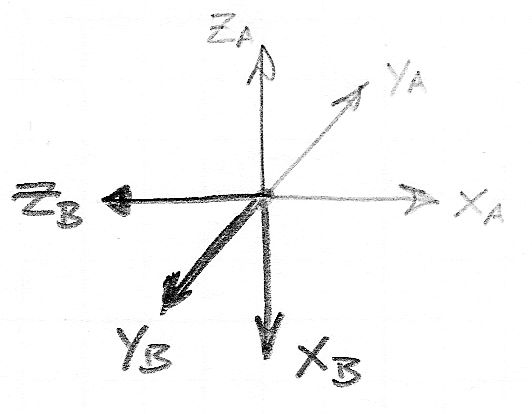
\includegraphics[width=1.5in]{00831.png}

Give the rotation matrix, $^A_BR$


\subsection{}
Two frames, $A, B$ start out superimposed.

1) Frame $B$ is rotated by $45^\circ$ around $Z_A$


2) Frame $B$ is rotated by $90^\circ$ around $X_B$


3) Frame $B$ is rotated by $30^\circ$ around $Y_B$

Find $^A_BR$

\subsection{}
Two frames, $A, B$ start out superimposed.

1) Frame $B$ is rotated by $23^\circ$ around $Y_B$


2) Frame $B$ is rotated by $67^\circ$ around $Z_A$


3) Frame $B$ is rotated by $16^\circ$ around $Y_B$

Find $^A_BR$


\subsection{}
A car has the same attached frame as Example 2.6 in the notes.  Its initial orientation is level, with $X_0$ pointing North.

1) It drives up a $30^\circ$ ramp.

2) It turns left by $45^\circ$ (still on the ramp)

3) It turns about $Z_0$ until it's compass reads straight West.


Find $^0_3R$

{\bf Warning - tough problem!}

\subsection{}
The car of Example 2.6

1) Drives forward 10 meters

2) turns left by $60^\circ$

3) drives in reverse for 5m

4) turns right $90^\circ$ and drives forward 6m

5) goes down a ramp at $30^\circ$ angle for 3m

Assume that when the car turns it does not displace at all (not true of real cars!).

Find the 4x4 homogeneous transform $^0_5T$ whcih representes the final position and orientation

\newpage
\subsection{}
An industrial robot must put individual chocolates in a box, $B$, which sits on table, $T$.   The box is located on a table with laser scanner, $S$. 

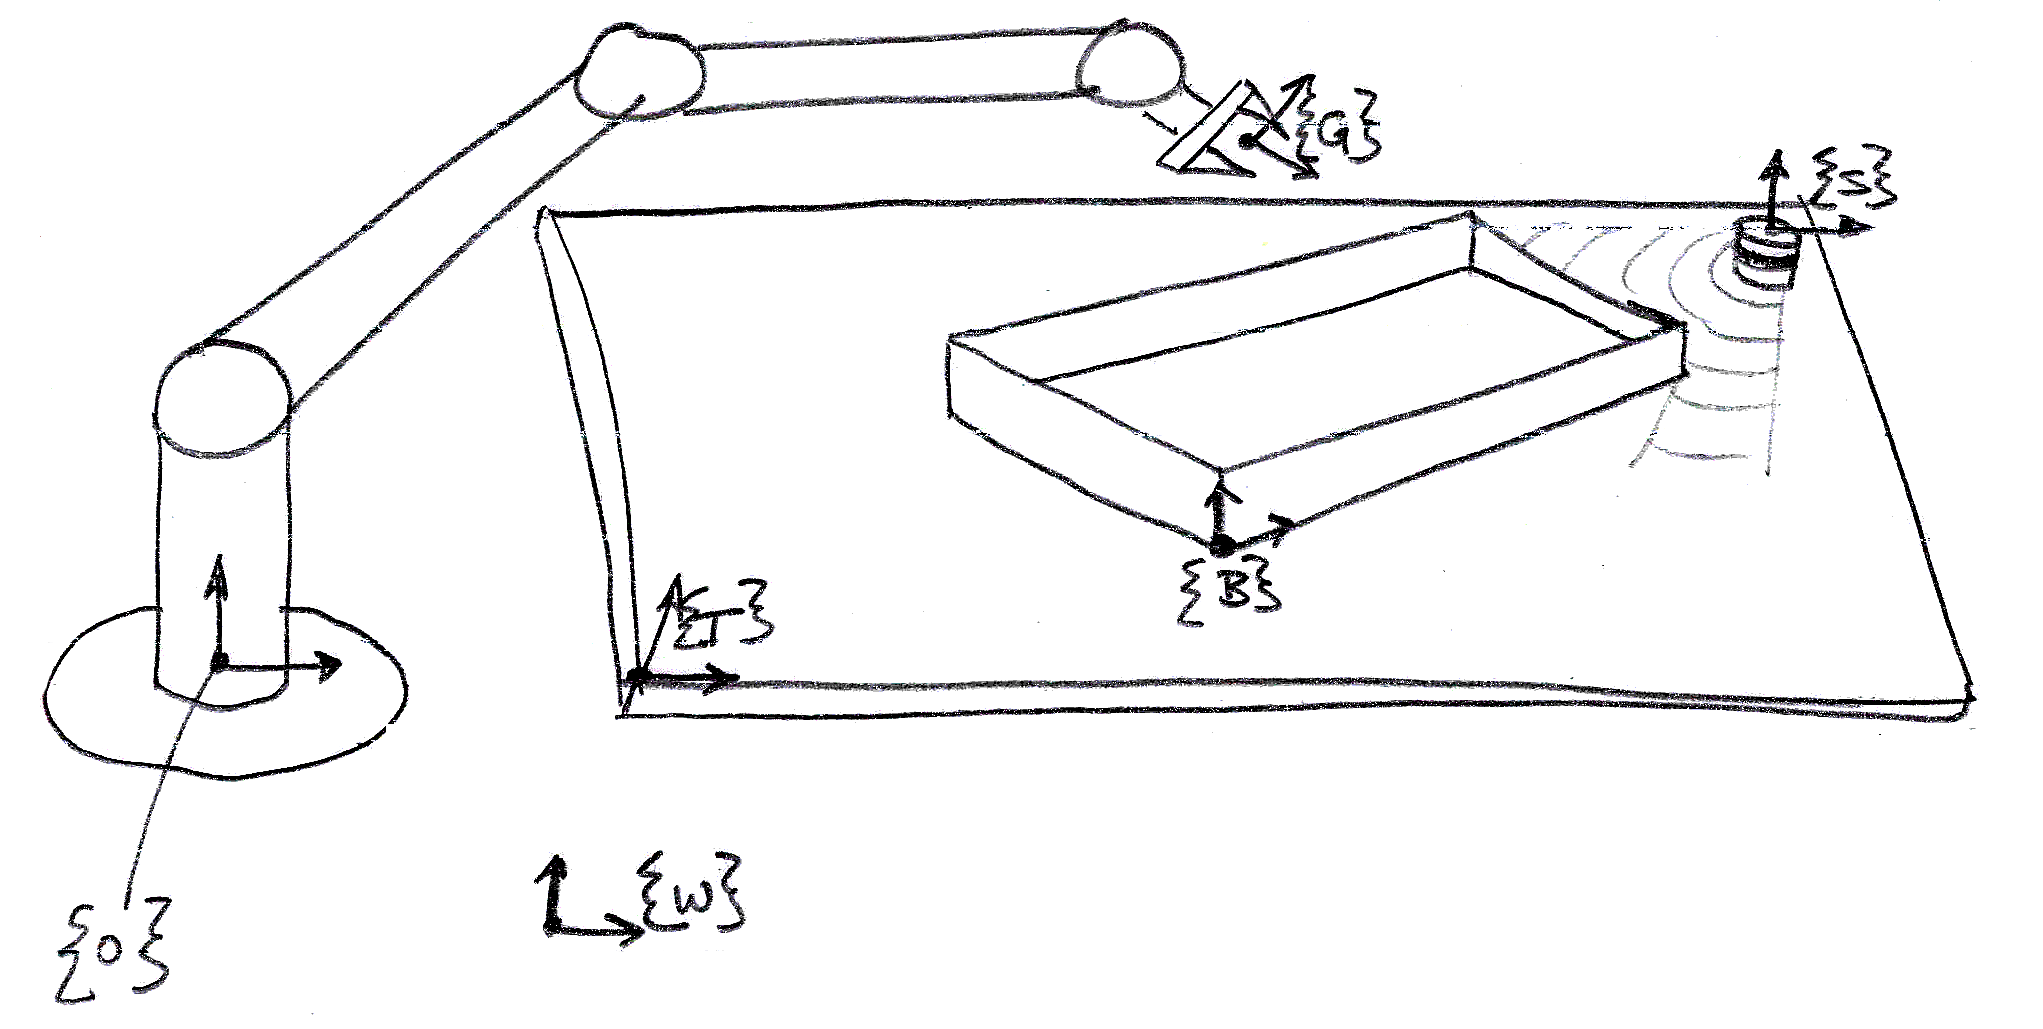
\includegraphics[width=6.5in]{hw1_543_W13_p6a.png}

The following relationships are known:

\[
{^O_GT}\quad{^O_WT}\quad{^T_WT}\quad{^T_ST}\quad{^S_BT}
\]

\subsubsection{}
Draw the transform graph.

\subsubsection{}
Find ${^O_BT}$



\end{document}

